\chapter{The Undepleted Region}\label{chap:bubble}

When simulating the detector using the impurity profile provided by the manufacturer, the simulated and measured depletion voltage often do not match. Given the large uncertainties in net impurity, the impurity profile may be scaled to bring these two values into agreement. This approach, which can be equated to a one-point calibration, provides a better estimate of the impurity profile, and is standard procedure in Ge detector simulation. Nevertheless, the simulated depletion voltage is highly degenerate, as many impurity profiles may lead to the same depletion voltage. For example, increasing the impurity concentration at the point-contact of a detector may be compensated by increasing the impurity gradient along the $\left<1\,1\,1\right>$-axis to lead to the same depletion voltage. 

A multiple-point calibration of the impurity profile can provide a much better estimate of the impurity profile. For undepleted detectors, the voltage dependence of the capacitance depends on the impurity profile of the detector. By measuring the CV (capacitance-voltage) curve of the detector and comparing it to simulation, the impurity profile of the detector can be fit using an arbitrary number of points. This has been done in a recent publication, where the deduced impurity profile contains both longitudinal and radial gradients~\cite{cv_impurities}.

The capacitance reflects the geometry of the undepleted region, which until recently has not been imaged. In this chapter, the first images of the undepleted region of a large-volume, non-segmented HPGe detector are presented. The geometry of the undepleted region at 900\,V and 1200\,V is then employed in the determination of the impurity profile, using a one-dimensional quadratic impurity model, in Chapter~\ref{chap:simulation}. 

\section{Energy Estimation}

The undepleted region can be modeled as an additional and often dominant RC component in the electronics chain (see Eq.~\ref{eq:first_order_low_pass}) leading to significantly longer pulse rise times~\cite{cv_impurities}. This is seen in Fig.~\ref{fig:Cs_energy_calculation_1200V}, where the waveform demonstrates the characteristic response to a RC-integrator.  
\begin{figure}[htb]
    \centering
    \includegraphics[width=6in]{figs/bubbles/Cs_energy_calculation_1200V.png}
    \caption{The maximum of the trapezoidal filtered waveform (red) is used to estimate the energy for resting baseline and soft pileup events at 1200\,V bias. The resulting spectra is shown on the right with the fits described in the text.}
	\label{fig:Cs_energy_calculation_1200V}
\end{figure}

To avoid ballistic deficit, and taking the much higher noise levels into consideration, the energy estimation procedure was modified. The uncalibrated energy was estimated from the maximum of a 4\,$\upmu$s-8\,$\upmu$s-4\,$\upmu$s trapezoidal filtered waveform. This procedure is also exemplified at the left of Fig.~\ref{fig:Cs_energy_calculation_1200V}. Similar to when the detector is fully depleted, the soft pileup waveforms were decay corrected before energy estimation. The \CsS{} 662\,keV peak was used to perform a one-point energy calibration for the soft pileup and resting baseline populations separately. The fit function used for the calibration is also slightly modified and is given by Eq.~\ref{eq:energy_peak_fit} (with $f = 0$) plus a quadratic background component. These fits are shown on the right of the figure. Note that due to the high noise levels, the precise selection of soft pileup presented in Sec.~\ref{sec:pileup} was not used. Instead, all events with baseline offsets above the baseline mode were classified as soft pileup. 

The FWHM at 662\,keV is 18.4\,keV and 24.8\,keV at 900\,V and 1200\,V respectively for resting baseline events. The resolution of soft pileup events is very similar.

\section{Modifications to Analysis Pipeline}

Both camera modules were used to image the ICPC at 900\,V and 1200\,V. Since these measurements were not intended for pulse shape analysis, and the presence of noise bursts did not affect the energy resolution, the up to 100\% increase in statistics given by the second camera was capitalized on. Using the coordinate transformation in Eq.~\ref{eq:czt_relative3D}, the hit positions in the second camera were placed in the coordinate system of the first and both data streams were merged. This allowed for the data of the second camera module to be seamlessly integrated into the established analysis pipeline. 

The pipeline was modified to account for the much poorer energy resolution of the detector at 900\,V and 1200\,V. The width of the contained event window was scaled for a bias, HV, such that events which satisfy 
\begin{equation}
	\left|E_\text{CAM} + E_\text{IC} - 662\,\text{keV}\right| \leq 8\,\text{keV}\frac{\text{FWHM(HV)}}{\text{FWHM(3500\,V)}}~,
\end{equation}
were selected for position reconstruction. The sum peak ($E_\text{CAM}+E_\text{IC}$) is used to calculate the FWHM. As seen in on the right Fig.~\ref{fig:z_reconstruction_energy_HV_1200}, this scaled energy window properly captures the contained Compton events on the diagonal of the two-dimensional histogram.
\begin{figure}[htb]
    \centering
    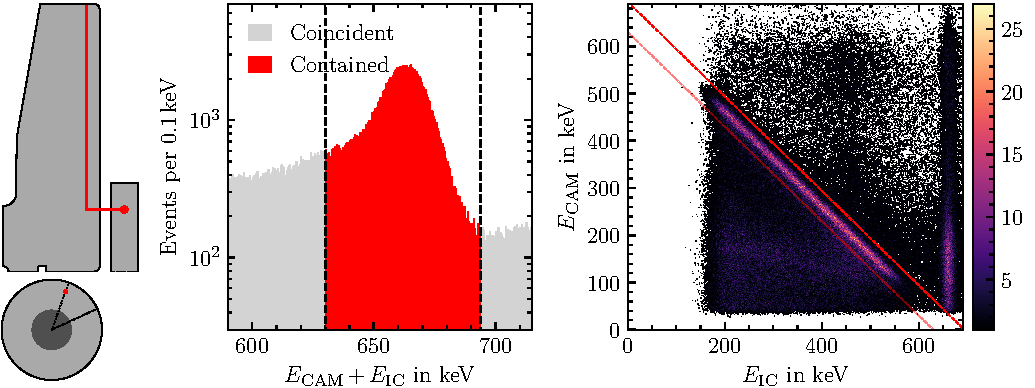
\includegraphics[width=6in]{figs/bubbles/z_reconstruction_energy_HV_1200.png}
    \caption{The sum energy peak and contained cut at 1200\,V is shown on the left. The events in the peak in red are the same as those in between the dashed red lines in the two-dimensional histogram on the right.}
	\label{fig:z_reconstruction_energy_HV_1200}
\end{figure}
Given that the data cleaning cuts were designed for depleted or near-depleted detector operating conditions, they could not be applied to the data taken at 900\,V and 1200\,V. Thus, only the LN$_2$ fill cut was applied. 

The position of the selected events was reconstructed with one final modification. Given the superior energy resolution of the camera in comparison with the undepleted ICPC, the energy of the camera was used for the calculation of the Compton angle:
\begin{equation} \label{eq:compton_CAM}
    \cos(\theta) = 1 - \dfrac{m_ec^2 E_\text{IC}}{662\,\text{keV} \times \left(E_\text{CAM}\right)}~.
\end{equation}
where $662\,\text{keV} - E_\text{IC}$ in Eq.~\ref{eq:compton_IC} has been replaced by $E_\text{CAM}$. Additionally, a camera energy cut, which restricts the Compton angle, $\theta$, to $(90\pm30)^\circ$ was applied. Similarly, only the energy of the camera was used for the $\alpha$-validation of 2-hit events (right-hand-side expression of Eq.~\ref{eq:compton_alpha}). In this manner, the energy of the detector was only used for event selection, leaving the upper limit in position reconstruction resolution (2\,mm) unaltered. Nevertheless, wider contained event windows were needed due to the poor detector energy resolution at 900\,V and 1200\,V. Therefore, a greater contamination of misreconstructed events is expected.
\begin{figure}[htb]
    \centering
    \includegraphics[width=6in]{figs/bubbles/bubble_rates.png}
    \caption{Effective Compton capture rate for (from left to right) 1-hit events with the detector at 3500\,V and 1200\,V bias and 2-hit events with the detector at 3500\,V and 1200\,V bias along the $\left<1\,0\,0\right>$ axis of the detector. The scan at 3500\,V was performed with the same camera positions (shown in the pictogram) as the 1200\,V scan.}
	\label{fig:bubble_rates}
\end{figure}

The effective Compton capture rate was calculated from Eq.~\ref{eq:effectve_compton_capture_rate}, with all the cut efficiencies, except LN$_2$, set to unity. To image the depletion surfaces, a reference rate at full depletion bias was needed. Thus, a dedicated measurement was performed at 3500\,V. For a fair rate comparison, both cameras were employed, using the same camera positions at a given \CsS{} source position that at 900\,V and 1200\,V. Although not a necessary condition, similar measurement time were also used. Even though at 3500\,V the detector energy resolution is better than the camera's, the position reconstruction was carried out using the procedure outlined in this section. The same event selection criteria was also followed. $\mathcal{R}^c$ is shown for the reference data taken at 3500\,V and the undepleted data taken at 1200\,V in Fig.~\ref{fig:bubble_rates}. 

\section{Depletion Surfaces}

The effective Compton capture rates at 900\,V and 1200\,V were divided by the same 3500\,V reference rate to produce the images shown in Fig.~\ref{fig:bubbles}.
\begin{figure}[htb]
    \centering
    \includegraphics[width=6in]{figs/bubbles/bubbles.png}
    \caption{$\mathcal{R}^c_{900\,\text{V}}/\mathcal{R}^c_{3500\,\text{V}}$ and $\mathcal{R}^c_{1200\,\text{V}}/\mathcal{R}^c_{3500\,\text{V}}$ is shown for the $\left<1\,0\,0\right>$ axis of the detector on the left and right respectively. For each bias the rate ratio calculated from 1- and 2-hit events is shown on the left and right respectively.}
	\label{fig:bubbles}
\end{figure}

A clear depletion surface, identifiable as a strong underfluctuation in blue in the center of the arm extending towards to point-contact, is seen at 900\,V to 1200\,V. The surface is present across the 1- and 2-hit event heat maps and shrinks as expected with higher bias. As opposed to $\mathcal{R}^c_{3100\,\text{V}}/\mathcal{R}^c_{3500\,\text{V}}$ (see Fig.~\ref{fig:bubble_3100}), where on average a near unity ratio is obtained everywhere in the bulk except the depletion surface, a persistent and constant overfluctuation is seen in Fig.~\ref{fig:bubbles} surrounding the depletion surfaces. Since these active regions are mostly featureless, the overfluctuation is hypothesized to originate from a greater number of misreconstructed events at 900\,V and 1200\,V with respect to when the detector is close to or at full bias voltage. Note that this follows from the wider contained event window used for the lower biases.

The average 2-hit event $\mathcal{R}^c_{\text{HV}}/\mathcal{R}^c_{3500\,\text{V}}$, with $\text{HV} = (900, 1200, 3100)$\,V in the active region of the detector is 1.61, 1.56 and 0.98 respectively. Assuming the overfluctuations in the active regions are constant over the entire volume, the heatmaps can be corrected. Dividing the rate ratios by their respective active region averages produces the final images of the evolution of the depletion surface, shown in Fig.~\ref{fig:bubbles_prog}.
\begin{figure}[htb]
    \centering
    \includegraphics[width=6in]{figs/bubbles/bubbles_prog.png}
    \caption{The corrected $\mathcal{R}^c_{\text{HV}}/\mathcal{R}^c_{3500\,\text{V}}$ is shown at $\text{HV} = (900, 1200, 3100)$\,V (from left to right) for the $\left<1\,0\,0\right>$ axis of the detector. The heatmaps have been mirrored to include the (unscanned) radial slice at $\phi+180^\circ$.}
	\label{fig:bubbles_prog}
\end{figure} 